\chapter{Methodology}

Based on our related work, describe (using the goals outlined in the beginning) the approach I take:
creating a better model to be used in carbon-aware scheduling 
using the model and evaluating it.
\section{Improving the current Job model}

We should probably argue why the current job model used in literature is not sufficient (WaitAWhile\cite{wiesner_lets_2021} assumed constant power usage and no overhead from stopping and resuming)

\subsection{Power Measurements on Machine Learning Jobs}
\label{sec:power_measurements}

\todo{Für die Durchführung von Messungen ist es zwingend erforderlich, die verwendete Testumgebung (Hardware wie auch Software) zu dokumentieren sowie Messparameter gewissenhaft zu wählen. Zu den wichtigsten Parametern gehren die Anzahl der Messwiederholungen, die Anwendung von Warmup-Läufen sowie die Identifikation und Vermeidung möglicher störender Einflüsse.}

\todo{I feel like I should add a paragraph somewhere explaining what I want to measure}

\paragraph{Options for measuring power}

There are multiple options for measuring the power of a given computer. One way of classifying these options would be under them being either \emph{logical measurements} or \emph{physical measurements}.

Logical ones would create a model on some metrics and derive the used power. One example would be using Linux' \emph{perf} tool to read hardware performance counters. \todo{This needs some more here}

Advantages of choosing a logical approach would be that no external hardware is needed and that the overhead of the measurement would be low, as the hardware counters are being kept track of anyway. Disadvantages on the other hand would be that such a model would have to be created or chosen and would include some form of error as all models do.

Physical measurements follow another route; measurement devices would be put between the operating hardware and the power supply. The point where a power measuring device is inserted would dictate what could and could not be measured, a wall mounted measurement device could only measure all power going into a computer and not differentiate between individual programs.

Advantages of physical measurements are that they can give a more holistic measurement of a system as would be the case for a wall mounted measurement device. Portability is an issue however, unlike operating-system supported tools such as perf, a measurement device would need more effort to be used on another system (or be entirely not useable, for example when such devices are only rated for a certain power level).

Due to having a power-measurement tool on-site in our university and it allowing whole-system measurements directly, I chose to follow the physical measurement option. 

\paragraph{Measurement tool}

The concrete tool used is the \emph{Microchip MCP39F511N Power Monitor (henceforth called MCP)}, which can be inserted between the device to test and the wall mounted power supply. A picture of it can be found in figure \ref{fig:mcp}. The MCP can report the current power consumption in 10 mW steps, each 5ms.

\begin{figure}
    \missingfigure{A figure of the MCP, ask Sven about this}
    \caption[short]{The MCP}
    \label{fig:mcp}
\end{figure}

\todo{I could include an extra paragraph on why the MCP is cool, and what it does differently, perhaps. Was there anything cool? I vaguely remember some measurement devices having two capacitors to more accurately determine usage}

I then used \emph{pinpoint}, a tool for energy profiling that can use different inputs, among them being the MCP, to read out its data. 

\paragraph{The test environment}

The experiments were run on my personal computer, the components of that are listed via the \emph{hwlist} tool, with unnecessary columns and rows being redacted for brevity:

\begin{lstlisting}[language=bash, frame=single, numbers=none, caption={Hardware that was measured}, basicstyle=\ttfamily]
   $ lshw -short -C processor -C memory -C display -C bus
Class          Description
==========================
bus            AB350 Gaming K4
memory         16GiB System Memory
processor      AMD Ryzen 5 1600X Six-Core Processor
display        GP104 [GeForce GTX 1070]
\end{lstlisting}

Information about the operating system is given via \emph{hostnamectl}, again some parts redacted:

\begin{lstlisting}[language=bash, frame=single, numbers=none, caption={Used operating system information}, basicstyle=\ttfamily]
    $ hostnamectl 
   Operating System: Ubuntu 24.04 LTS                
             Kernel: Linux 6.8.0-39-generic
\end{lstlisting}

\paragraph{Measured Program}

Machine learning (ML) was used as the main motivation for checkpoint \& resume scheduling in the related works\cite {wiesner_lets_2021} and thus was also chosen by me to be measured and modeled. 

The concrete model and framework is secondary for our measurement. In my case, a small model would be chosen in order to have fewer data points for processing as well as faster iterations on the measurement script. 

There is a vast amount of machine learning frameworks. For a high-level model, the feature set of the framework only needed to support checkpointing, resuming, and some basic form of logging. 
Glancing at the documentation of popular frameworks such as \emph{torch}, \emph{tensorflow}, and \emph{huggingface} shows that these features are commonly supported. 

With not much bias towards any framework, huggingface was chosen because my supervisor Felix supplied a sample "hello-world"-esque machine learning script for python \emph{roberta.py}\footnote{\url{https://github.com/Quacck/master-thesis/blob/main/power-measurements/roberta.py}}.

The huggingface trainer supports callbacks, I thus modified the code by adding timestamped logs. These "Events" would be output into another .csv File I could later use.\todo{Later use for WHAT?!}

\paragraph{Conducted Experiments}

A script \footnote{\url{https://github.com/Quacck/master-thesis/blob/main/power-measurements/measure_roberta.sh}} was created to execute each experiment. 

On a high-level view, the following experiments were conducted: 

\begin{enumerate}
    \item \label{experiment:full}Run the whole program start to finish
    \item \label{experiment:partial_checkpointed}Run it partially, checkpointing after some step, sleeping, resuming from that step
    \item \label{experiment:partial_checkpointed_aborted}Run it partially, checkpointing after some step but aborting before the next checkpoint. Then resume as above.
    \item \label{experiment:startup_only}Run only the startup phase up until the ML would start
    \item \label{experiment:baseline}Do nothing, measure the system at rest
\end{enumerate}

Experiment \ref{experiment:full} would give a baseline for what the job would look like without checkpoint \& resume. Number \ref{experiment:partial_checkpointed} and \ref{experiment:partial_checkpointed_aborted} would be used to determine the overhead of checkpointing the job. \ref{experiment:startup_only} would be used to validate the other ones. The last experiment is necessary to determine the baseline energy consumption of the environment.

To execute these experiments inside a repeatable bash script, additional command line parameters were added to the given python script. 
For example, there would be a boolean parameter \verb|--resume_from_checkpoint|, or an integer parameter \verb|--stop_after_epoch| would be used for experiment \ref{experiment:full} to \ref{experiment:partial_checkpointed}. 
The way of doing experiment \ref{experiment:startup_only} was to copy the script, and delete everything after the imports.

\paragraph{Creating repeatable measurements}

As this is being run on standard hardware on a standard operating system, all experiment are subject to noise. 
For example, \emph{Dynamic frequency and voltage scaling (DFVS)}, the OS technique of increasing CPU "speeds" according to work load would add power in an uncontrolled way. Also, background tasks may happen "randomly", increasing power usage. 

Thus, for the testing, any foreground apps would be closed. I also used \emph{cpupower}, as shown in snippet below, to set the CPU frequency to a set value:

\todo{Think about whether this is really interesting, I guess keep it if I need more content}
\todo{What is the MAXFREQ of my ryzen 5?}
\begin{lstlisting}[language=bash, frame=single, numbers=none, caption={Used operating system information}, basicstyle=\ttfamily]
    MINFREQ=$(cpupower frequency-info --hwlimits | sed -n '1d;p' \
        | awk '{print $1}')
    MAXFREQ=$(cpupower frequency-info --hwlimits | sed -n '1d;p' \
        | awk '{print $1}')
    
    cpupower frequency-set --min ${MAXFREQ} &>/dev/null
    cpupower frequency-set --max ${MAXFREQ} &>/dev/null

    # ... conduct experiments

    cpupower frequency-set --min ${MINFREQ} &>/dev/null
    cpupower frequency-set --max ${MAXFREQ} &>/dev/null
\end{lstlisting}
\label{listing:setting_cpu_frequency}

As machine learning makes use of available GPUs, the frequency should also be similarly set to a defined value. 
NVIDIA provides guide on how to do so \footnote{\url{https://developer.nvidia.com/blog/advanced-api-performance-setstablepowerstate}}.
Sadly, my used GPU, the NVIDIA GTX 1070, is not capable of fixing the frequency as of the time of conducting these experiments. 
While it is supposed to be possible according to SOURCE\todo{Reconstruct this argument, perhaps theres still something in my PC history | grep}, but there seems to currently be drivers issue preventing this\todo{Find the forum post of people complaining}. 
Thus, the frequency of the GPU was not fixed. 
To reduce the effect of frequency scaling here, the time between experiments was increased generously so that any impact from such scaling would reoccur throughout each run and there would be reduced dependency between runs.

\todo{further explain how the experiments were conducted}

\paragraph{Conducting each experiment}

Each experiment was re-run 10 times. Between each run, there would be a \verb|sleep| period of 10 seconds and one of two minutes in the partial executions. 
Additionally, \verb|pinpoint|'s feature of measuring before and after the actual program-to-test would be used. 
This leads to a period of 30 seconds being measured around the actual experiment. 
Plotting these additional time frames would give a quick visual indicator whether experiments are sufficiently isolated from each other, ergo when the power draw is at the baseline as the actual program starts.

As there is some data being downloaded and persisted during the execution of the ML, before each run, the data would be cleaned up.

\paragraph{Collected data}

For each experiment, a named and timestamped folder would be created in the \verb|/power-measurements| folder of my repository. Each folder would then hold a \verb|.csv| with pinpoint's timestamped power measurements. 
The added timestamped-logging would be saved into another \verb|.csv|. 
While figuring out how to conduct the experiments, I would then plot these measurements early and visually spot if there were any obvious errors or mistakes.

\paragraph{Determining the baseline power draw}

Beginning with the most exiting experiment, determining the baseline and testing the amount of the underlying environment. 
One sample run is shown in Figure \ref{fig:plot_baseline}.
The blue dots in figure represent each data point. The red line is a smoothed Gaussian trend line with $\sigma = 2$. 
Dark-green vertical lines are the logged or derived "events" for each run. In this case, nothing happens, so it is only the start and end of \verb|sleep 120|. 
Notice how the trace starts 30 seconds before the start and continues for another 30 seconds because of the aforementioned \verb|pinpoint| feature.
Going further, these additional measurements will be redacted for brevity, unless something worth mentioning happens outside the actual experiments.\todo{Check later if something interesting happens or if I should reword this.}

\begin{figure}
    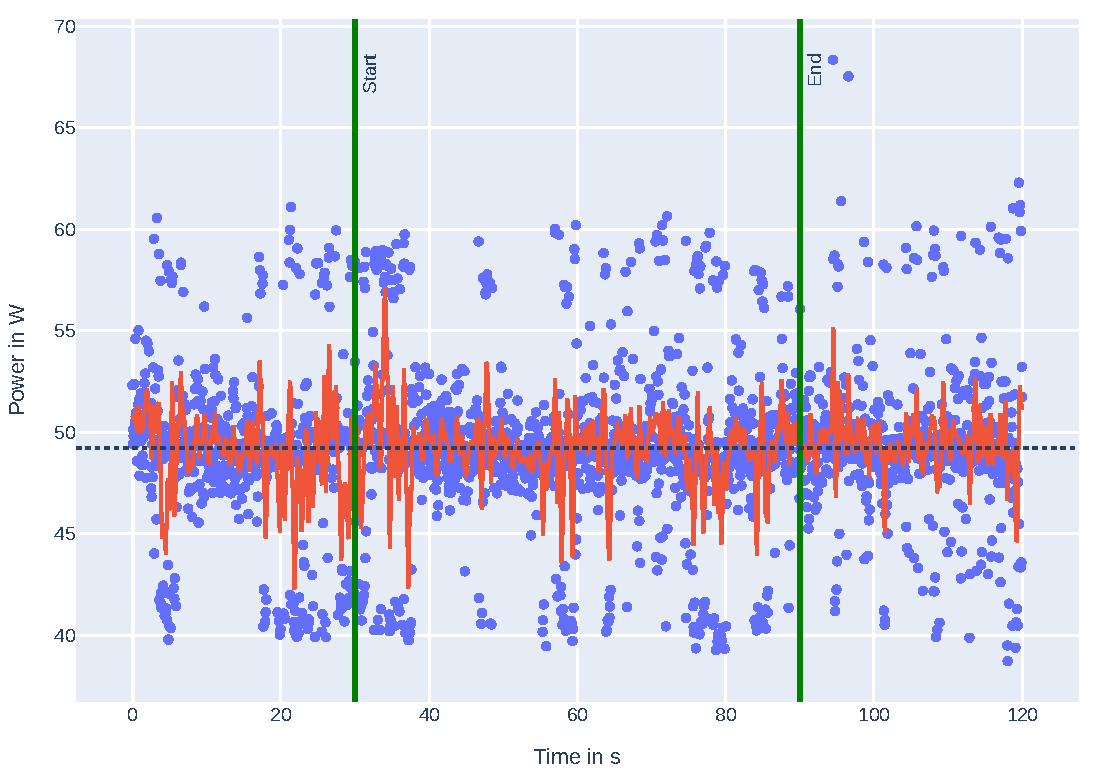
\includegraphics[width=\linewidth]{power-measurements/measurements_sleep_0714004033/plot.pdf}
    \caption{Sample run of the baseline experiment}
    \label{fig:plot_baseline}
\end{figure}

Across all 10 runs, the average baseline power draw is calculated via the mean of all data points. This comes out as an average of 49.8 W with a standard deviation of 4.4 W.

The baseline power draw will be less interesting going further, but will put perspective on the power draws of the other experiments. The standard deviation should gives a broad idea of how much noise is in the system environment.

\paragraph{The non-interrupted run}

\begin{figure}
    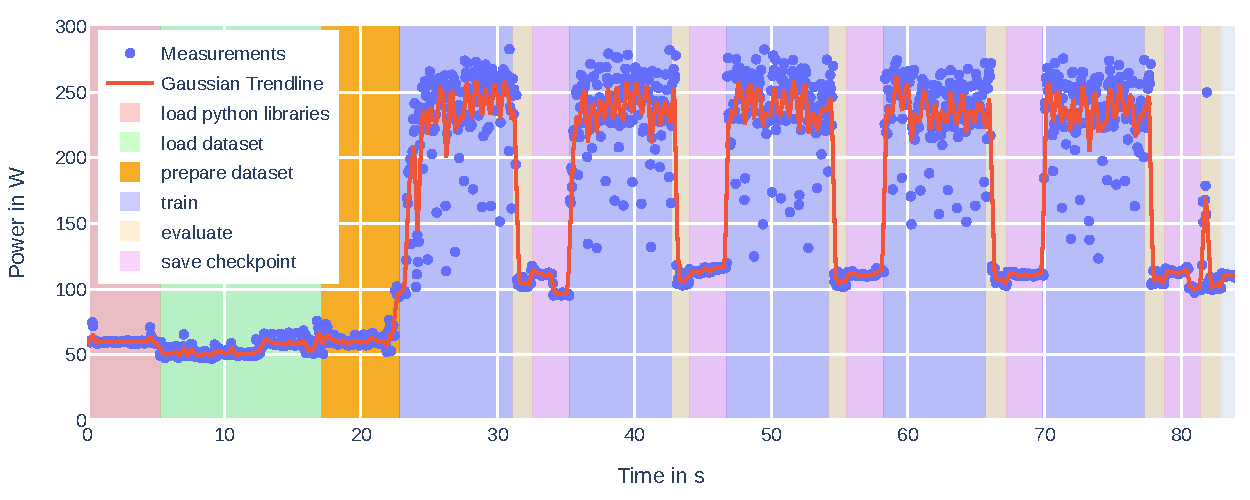
\includegraphics[width=\linewidth]{power-measurements/measurements_roberta_full_0714010405/plot.pdf}
    \caption{Sample run of the full run experiment}
    \label{fig:plot_full}
\end{figure}

\begin{itemize}
    \item Warum ist das interessant
    \item which jobs did I measure and why?
    \item Wie habe ich die Messungen ausgeführt, MCP beschreiben, sowie pinpoint als Schnittstelle
    \item Experimentier-parameter, also wodurch versuche ich sicherzustellen, dass meine Messungen auch sinn machen / reproduzierbar sind usw usw.
    \item Wie habe ich das ausgewertet, schöne graphs zeigen
\end{itemize}

\subsection{Defining a new model}

Now that we know what a high-level job looks like, we can pick it apart and reduce the real-world measurements of one program to a more generic model. 

\begin{itemize}
    \item we can deduce phases
    \item each phase has a constant power draw
    \item give an example of how to represent the real-world measurements into a model
    \item now we should proof that the model actually represents the reality to a certain degree (error analysis)
    \item have a cute graph showing the measurements and the model-"measurements" next to each other
    \item also show that the stop-resuming functionality can be represented with our model
\end{itemize}

\section{Choosing an implementation approach}

We first need to explain why we chose our approach (building upon exisiting work inside GAIA). The other option that is not using a simulation would be to schedule real jobs, for example by creating a slurm plugin.

We can then evaluate how well a slurm plugin would work for our given Forschungsragen. End that section by deeming the plugin idea as unfit, we can then shift to arguing for the simulation approach as that is also something that just came out in related work (perhaps we should see wether we list GAIA as related work or introduce it just then)

\subsection{Carbon-aware scheduling via a slurm plugin}
\label{subsec:slurm_plugin}

thank god I made notes

\begin{itemize}
    \item why do we choose slurm specifically, and not other software like kubernetes etc. => because its also being used in scorelab at the same location as I am in
    \item was ist slurm? => "open source, fault-tolerant, and highly scalable cluster management and job scheduling system for large and small Linux clusters"
    \item how does the slurm plugin system work? what do we need to do to get there?
    \item what problems occured?
    \item ...thus I ultimatly choose not to pursue implementing a plugin
\end{itemize}

\subsection{Using a Simulation approach}

Thankfully, just at that time a new paper \cite{hanafy_going_2024} was released. 
They made a prototype testbed for simulating job scheduling on cloud providers. These Jobs could be executed on spot instances (cheap VMs that seek to increase cloud utilization), on-demand instances (short-notices VMs that are thus more expensive) or pre bought VMs (medium cost, but may be wasted), the paper then discussed balancing carbon- and dollar costs.

The good part is that within that testbed, many scheduling approaches outlined in the related work section were implemented - a WaitAWhile Implementation for example \todo{improve this}. I could now extend this testbed and would ontop get something to compare against!

The way to do this section would be to a) describe what was already there, and b) what I changed

\missingfigure{This would show a class diagram similar to the one in the GAIA paper, with markings which files I edited / added / deleted}

Describe the figure, explain why I am for example removing the part about the dollar-costs and the slurm-scheduler adapter. I should also describe which parts of the program I am modifiying to tackle my Forschungsfragen


Stuff I should describe about the simulation before I added anything:

\paragraph{Assumptions of the simulation}

\begin{itemize}
    \item Joblängen sind bekannt
    \item Jobs können zeitlich verschoben werden (begründet daraus, dass sie als Batch Jobs submitted werden, andere Jobs werden hierbei nicht betrachtet)
    \item User geben dabei an, wie lange der Job verschoben werden darf
    \item Die carbon curve auf dem electrical grid ist für kurze Zeiträume in der Zukunft bekannt
    \item Die Hardware ist zZ nicht begrenzt. Das war in der related work auch nicht so. Eigentlich wäre es spannend sich das anzuschauen, allerdings sind die bisherigen Scheduler halt darauf garnicht gemünzt, da werden alle Jobs unabh. voneinander gescheduled. Man könnte das via publicCloud argumentieren, allerdings wäre das questionable, in wie fern der scorelab trace benutzt werden kann (da das ja auf in einem lokalem datacenter läuft)
    \item TODO: Joblängen sollten dem Scheduler nicht bekannt sein. Die Workloads aus GAIA werden allerdings so gescheduled als ob man perfekte Knowledge hat. Das reicht zwar für ein upper bound an carbon savings, ist aber nicht sehr realistisch.  
\end{itemize}

\paragraph{Data being used}

here i could describe which data is already being used (the traces, aswell as the historical carbon data)
\begin{itemize}
    \item Welche Traces gibt es, wodurch werden die characterisiert? (Länge, Anzahl, etc, etc) Vllt. kann man hier nen coolen vergleich erstellen, Auch könnte man ein paar Sätze darüber schreiben, wie die bisher in GAIA aufgenommen wurden.
    \item Wie den scorelab trace benutzen und übersetzen? Gerne auf ner halben Seite aufschlüsseln, was die einzelnen Attribute aus sacct bedeuten.
    \item Ansonsten kann man noch die dynamic ernergy sachen als Datenquelle auflisten, bzw. das mini experiment mit fmnist und roberta 
\end{itemize}


\section{building ontop of the existing gaia sim}

Which parts of GAIA do I add on?
=> this should just be the schedulers and the part where the carbon is calculated, this ensures that 

\section{Evaluating carbon-aware scheduling with the new job model}

Hi!